\documentclass[12pt,a4paper]{article}

\usepackage[T2A]{fontenc}
\usepackage[utf8]{inputenc}
\usepackage[russian]{babel}
\usepackage{amsmath,amssymb}
\usepackage{graphicx}
\usepackage{booktabs}
\usepackage{geometry}
\geometry{margin=2.4cm}
\usepackage{tikz}
\usetikzlibrary{arrows.meta,positioning,shapes.geometric}
\usepackage{float}
\usepackage{caption}
\captionsetup{labelsep=endash}
\usepackage{hyperref}
\hypersetup{colorlinks=true,linkcolor=black,urlcolor=blue}

\title{Лабораторная работа №\,1\\ \large Многомерная оптимизация сложной функции генетическим алгоритмом (функция Леви)}
\author{Панов Артемий, Б24-527}
\date{2026 г.}

\begin{document}
\maketitle

\section{Постановка задачи и индивидуальный вариант}

Требуется найти приближённое глобально оптимальное решение задачи
\[
\min_{\mathbf{x} \in D} f_V(\mathbf{x}), \qquad
\mathbf{x} = (x_1, \dots, x_d),
\]
генетическим алгоритмом с вещественным кодированием.

Индивидуальные параметры: $N = 18$ (порядковый номер в группе), $Q = 2$
(индекс группы 527), $Y = 26$ (год 2026). Номер варианта:
\[
V = 1 + \big((17N + 7Q + Y) \bmod 20\big) = 1 + (346 \bmod 20) = 7,
\qquad d = 5 + (V \bmod 6) = 6.
\]

\textbf{Вариант 7 --- функция Леви}, область поиска $-10 \le x_i \le 10$,
размерность $d = 6$.

\section{Целевая функция и её свойства}

Функция Леви:
\[
f(\mathbf{x}) = \sin^2(\pi w_1)
 + \sum_{i=1}^{d-1} (w_i - 1)^2\,\bigl[1 + 10\sin^2(\pi w_i + 1)\bigr]
 + (w_d - 1)^2\,\bigl[1 + \sin^2(2\pi w_d)\bigr],
\qquad w_i = 1 + \frac{x_i - 1}{4}.
\]

\textbf{Ориентир по глобальному минимуму} (требование задания для
вариантов 7 и 10): по литературным данным $f^* = 0$ в точке
$\mathbf{x}^* = (1, 1, \dots, 1)$ --- там все $w_i = 1$, первое слагаемое
$\sin^2(\pi w_1) = 0$, а все множители $(w_i - 1)^2$ обнуляются. Реализация
проверена: $f(\mathbf{1}) < 10^{-20}$.

Свойства ландшафта (рис.~\ref{fig:slice}):
\begin{itemize}
\item \textbf{мультимодальность}: множители $1 + 10\sin^2(\cdot)$ создают
  сетку локальных минимумов с периодом $\Delta w = 1$, то есть
  $\Delta x = 4$ по каждой координате (в последней --- $\Delta x = 2$);
  в $[-10, 10]^6$ это порядка $5^6 \approx 15\,000$ ячеек-ловушек;
\item \textbf{глобальная чаша}: суммы $(w_i - 1)^2$ дают грубый
  квадратичный уклон к $\mathbf{x}^* = \mathbf{1}$ --- на масштабе всей
  области ландшафт <<связен>> в сторону оптимума;
\item \textbf{масштаб}: впадина глобального минимума узка относительно
  области, случайное попадание в её окрестность маловероятно.
\end{itemize}

\begin{figure}[H]
\centering
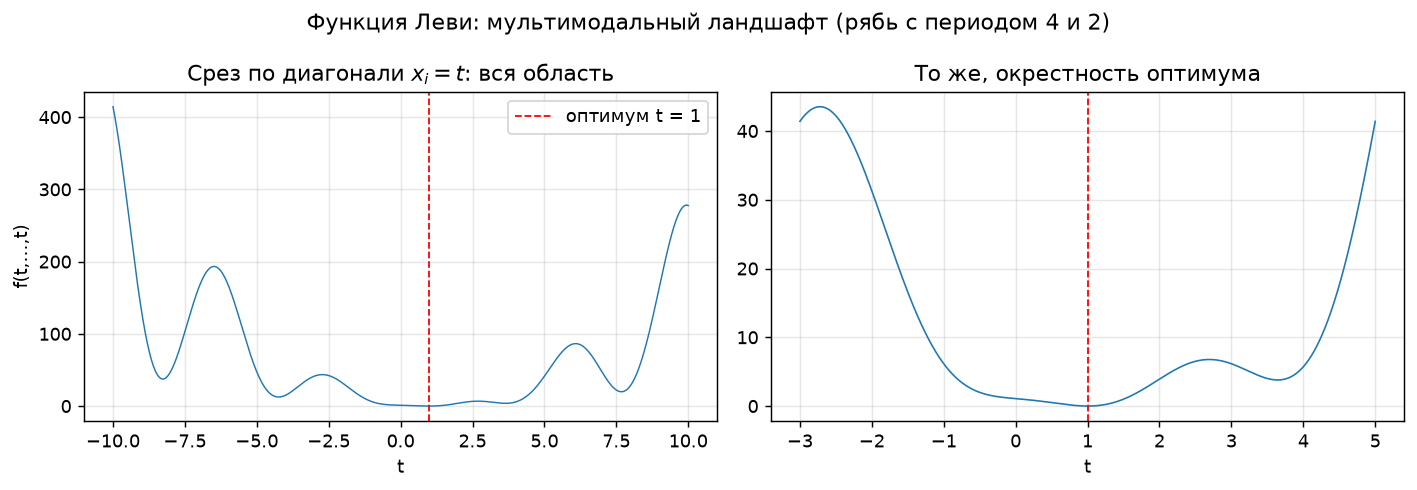
\includegraphics[width=0.98\textwidth]{figures/levy_slice.png}
\caption{Срез функции Леви по диагонали $x_i = t$: вся область (слева)
и окрестность оптимума (справа)}
\label{fig:slice}
\end{figure}

\section{Представление особи}

Особь --- вещественный вектор $\mathbf{x} = (x_1, \dots, x_6)$,
$x_i \in [-10, 10]$; генотип совпадает с фенотипом, декодирование не
требуется. Инициализация --- равномерное распределение в области.
Фитнес --- значение целевой функции (задача минимизации).

\section{Генетический алгоритм}

Схема работы --- на рис.~\ref{fig:ga}, параметры --- в
таблице~\ref{tab:params}.

\begin{figure}[H]
\centering
\begin{tikzpicture}[
  node distance=0.45cm,
  box/.style={draw, rounded corners=2pt, align=center, minimum width=6.4cm,
              minimum height=0.85cm, font=\small},
  dec/.style={draw, diamond, aspect=2.6, align=center, font=\small, inner sep=1pt},
  arr/.style={-{Stealth[length=2.5mm]}, thick}]
\node[box] (init) {инициализация: 80 особей, равномерно в $[-10,10]^6$};
\node[box, below=of init] (eval) {оценка: $f(\mathbf{x})$ для популяции};
\node[dec, below=of eval, yshift=-0.1cm] (stop) {бюджет $10^4$ исчерпан?};
\node[box, below=of stop, yshift=-0.3cm] (elite) {элитизм: 2 лучшие особи --- в потомство};
\node[box, below=of elite] (sel) {турнирная селекция родителей ($k = 3$)};
\node[box, below=of sel] (cross) {BLX-$\alpha$ кроссовер ($\alpha = 0{,}5$, $p_c = 0{,}9$)};
\node[box, below=of cross] (mut) {гауссова мутация ($p_m = 0{,}15$, $\sigma$); clip в $[-10,10]$};
\node[box, right=2.0cm of stop] (end) {конец: лучшая особь};
\draw[arr] (init) -- (eval);
\draw[arr] (eval) -- (stop);
\draw[arr] (stop) -- node[left, font=\small]{нет} (elite);
\draw[arr] (elite) -- (sel);
\draw[arr] (sel) -- (cross);
\draw[arr] (cross) -- (mut);
\draw[arr] (mut.west) -| ++(-1.4,0) |- (eval.west);
\draw[arr] (stop) -- node[above, font=\small]{да} (end);
\end{tikzpicture}
\caption{Блок-схема генетического алгоритма}
\label{fig:ga}
\end{figure}

\begin{table}[H]
\centering
\small
\caption{Параметры алгоритма}
\label{tab:params}
\begin{tabular}{ll}
\toprule
Параметр & Значение \\
\midrule
Размер популяции & 80 ($\ge 30$ по заданию) \\
Селекция & турнирная, $k = 3$ \\
Рекомбинация & BLX-$\alpha$ кроссовер, $\alpha = 0{,}5$ (доп. задание), $p_c = 0{,}9$ \\
Мутация & гауссова на ген, $p_m = 0{,}15$, $\sigma \in \{0{,}05;\,0{,}3;\,1{,}0\}$ \\
Обработка границ & отсечение (clip) в $[-10, 10]$ \\
Сохранение лучшего & элитизм, 2 особи \\
Критерий остановки & бюджет $10\,000$ вычислений $f$ (инициализация включительно) \\
Серия & 30 независимых запусков, $\text{seed} = 7000 + 19i$ \\
\bottomrule
\end{tabular}
\end{table}

\textbf{BLX-$\alpha$ кроссовер} (реализован как дополнительное задание):
для родителей $c_1, c_2$ ген потомка выбирается равномерно в
$[\,c_{\min} - \alpha I,\; c_{\max} + \alpha I\,]$, где
$I = |c_1 - c_2|$, $\alpha = 0{,}5$. Оператор одновременно наследует
родительские значения и разведывает окрестность между ними и за их
пределами.

\section{Обоснование выбора операторов}

Структура задачи: мультимодальный ландшафт с мелкой рябью
(период $\Delta x = 4$) поверх глобальной квадратичной чаши. Отсюда
требования к операторам:
\begin{itemize}
\item \textbf{турнирная селекция} ($k = 3$) --- умеренное давление:
  различия между соседними ячейками ряби велики (чаша), турнир их
  улавливает, но не вызывает мгновенной схлопки популяции;
\item \textbf{BLX-$\alpha$} вместо арифметического кроссовера: середина
  между двумя родителями из разных ячеек ряби может быть хуже обоих ---
  BLX-$\alpha$ с расширением $\alpha I$ позволяет потомку оказаться и
  в родительских, и в соседних ячейках, то есть выполняет грубую
  разведку без разрушения уже найденных координат;
\item \textbf{гауссова мутация} --- локальная доводка координат; её
  масштаб $\sigma$ --- исследуемый фактор работы;
\item \textbf{элитизм} --- гарантия, что найденная доводка не теряется
  при рекомбинации;
\item \textbf{clip} --- простая и достаточная обработка границ для
  выпуклой (параллелепипед) области: оптимум лежит внутри, отражение
  не требуется.
\end{itemize}

\section{Методология эксперимента}

Три конфигурации отличаются \emph{только масштабом мутации}
$\sigma \in \{0{,}05;\ 0{,}3;\ 1{,}0\}$ (период ряби $\Delta x = 4$:
конфигурации покрывают режимы <<много меньше>> / <<заметная доля>> /
<<четверть периода>>). Для каждой --- 30 независимых запусков
($\text{seed} = 7000 + 19i$), бюджет $10\,000$ вычислений функции
у всех конфигураций, включая контроль случайным поиском. Фиксируются:
лучшее $f$ запуска, кривая лучшего значения, разнообразие популяции
(среднее СКО по координатам), время. По серии --- минимум, среднее,
медиана, стандартное отклонение, максимум.

\section{Результаты}

\subsection{Влияние масштаба мутации}

\begin{table}[H]
\centering
\small
\caption{Итоговое $f$ по 30 запускам для трёх масштабов мутации}
\label{tab:sigma}
\begin{tabular}{lccccc}
\toprule
Конфигурация & Лучшее & Среднее & Медиана & Стд & Худшее \\
\midrule
$\sigma = 0{,}05$ & $3{,}1{\cdot}10^{-8}$ & $2{,}9{\cdot}10^{-7}$ & $2{,}1{\cdot}10^{-7}$ & $2{,}1{\cdot}10^{-7}$ & $8{,}4{\cdot}10^{-7}$ \\
$\sigma = 0{,}3$ & $1{,}5{\cdot}10^{-6}$ & $1{,}1{\cdot}10^{-5}$ & $9{,}2{\cdot}10^{-6}$ & $6{,}1{\cdot}10^{-6}$ & $2{,}4{\cdot}10^{-5}$ \\
$\sigma = 1{,}0$ & $1{,}5{\cdot}10^{-5}$ & $1{,}0{\cdot}10^{-4}$ & $9{,}0{\cdot}10^{-5}$ & $5{,}7{\cdot}10^{-5}$ & $2{,}2{\cdot}10^{-4}$ \\
\bottomrule
\end{tabular}
\end{table}

\begin{figure}[H]
\centering
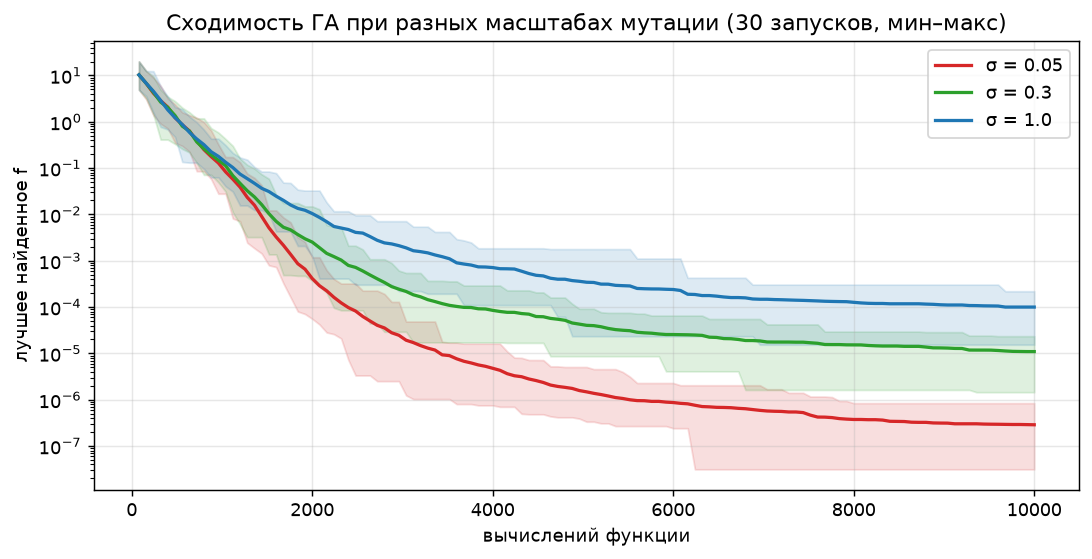
\includegraphics[width=0.86\textwidth]{figures/convergence_sigma.png}
\caption{Сходимость при разных $\sigma$: среднее и коридор мин--макс (30 запусков)}
\label{fig:conv}
\end{figure}

Все три конфигурации во всех запусках сходятся к глобальному минимуму,
но влияние масштаба мутации монотонно: чем меньше $\sigma$, тем точнее
результат --- среднее $f$ меняется
$2{,}9{\cdot}10^{-7} \to 1{,}1{\cdot}10^{-5} \to 1{,}0{\cdot}10^{-4}$
(рис.~\ref{fig:conv}). Объяснение: грубую разведку области выполняет
BLX-$\alpha$ кроссовер (его охват в разнообразной ранней популяции
перекрывает ячейки ряби целиком), а глобальная чаша $(w_i - 1)^2$ задаёт
отбору направление к оптимуму. Мутации остаётся роль доводки, поэтому
мелкий шаг выигрывает; крупный ($\sigma = 1{,}0$, четверть периода ряби)
постоянно сталкивает найденные координаты и ограничивает точность
уровнем $\sim 10^{-4}$.

\begin{figure}[H]
\centering
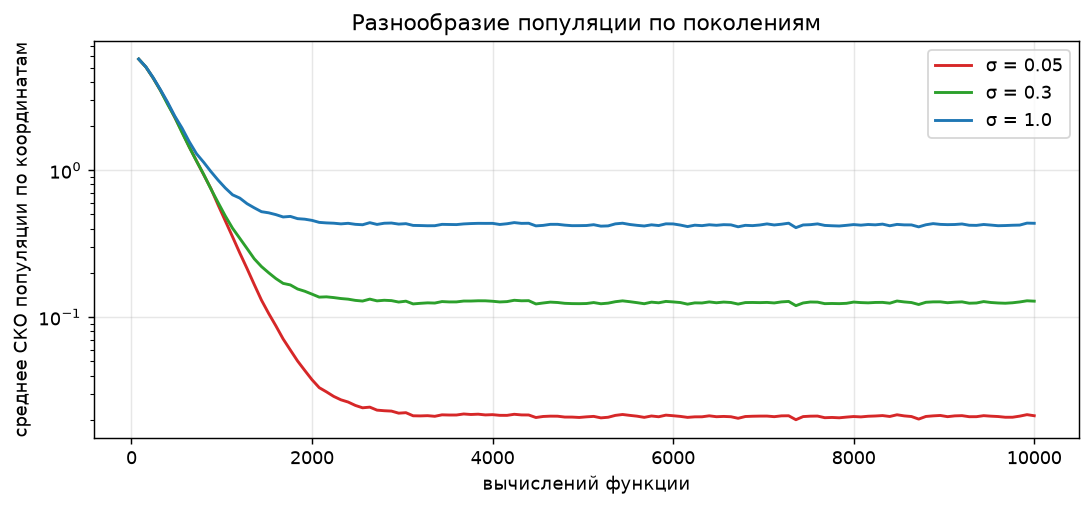
\includegraphics[width=0.82\textwidth]{figures/diversity.png}
\caption{Разнообразие популяции (среднее СКО по координатам)}
\label{fig:div}
\end{figure}

\textbf{Диагностика преждевременной сходимости.} Разнообразие падает у
всех конфигураций (рис.~\ref{fig:div}), при $\sigma = 0{,}05$ --- до
равновесного уровня $\sim 0{,}02$, задаваемого мутацией. Однако
сходимость не оказывается преждевременной в смысле остановки в чужой
ячейке: популяция схлопывается вокруг глобального оптимума
($f \sim 10^{-7}$). Причина --- связность ландшафта на грубом масштабе:
рябь Леви не перевешивает чашу, и правильная ячейка видна отбору из
любой точки области.

\subsection{Сравнение со случайным поиском}

\begin{table}[H]
\centering
\small
\caption{ГА (лучшая конфигурация) против случайной выборки, бюджет $10^4$}
\label{tab:vsrandom}
\begin{tabular}{lccccc}
\toprule
Метод & Лучшее & Среднее & Медиана & Стд & Худшее \\
\midrule
ГА, $\sigma = 0{,}05$ & $3{,}1{\cdot}10^{-8}$ & $2{,}9{\cdot}10^{-7}$ & $2{,}1{\cdot}10^{-7}$ & $2{,}1{\cdot}10^{-7}$ & $8{,}4{\cdot}10^{-7}$ \\
Случайный поиск & $0{,}96$ & $1{,}98$ & $1{,}85$ & $0{,}71$ & $3{,}73$ \\
\bottomrule
\end{tabular}
\end{table}

\begin{figure}[H]
\centering
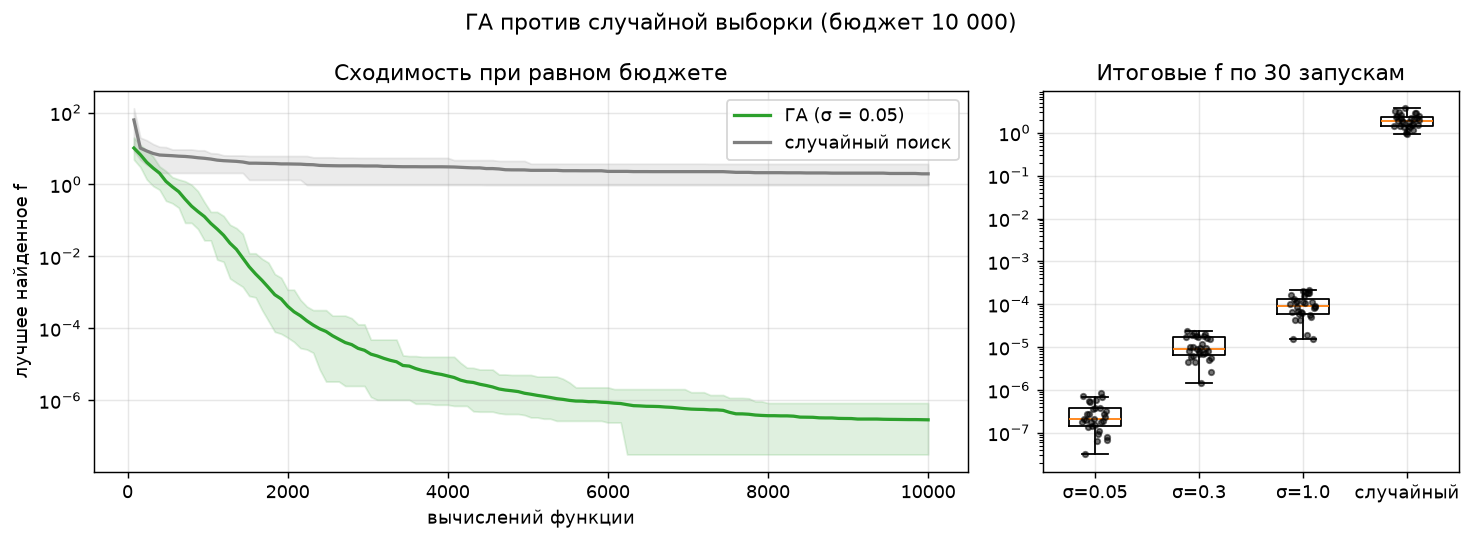
\includegraphics[width=0.98\textwidth]{figures/ga_vs_random.png}
\caption{Сходимость при равном бюджете (слева) и итоговые $f$ серий (справа)}
\label{fig:vsrand}
\end{figure}

При равном бюджете случайная выборка хуже ГА на \textbf{семь порядков}
(таблица~\ref{tab:vsrandom}, рис.~\ref{fig:vsrand}): объём окрестности
глобального минимума ничтожен в объёме $20^6$, и лучшая из $10^4$
случайных точек остаётся далеко за пределами доводки.

\textbf{Почему функция сложна для простого поиска.} Локальный спуск из
случайной точки останавливается в ближайшей впадине ряби (до неё ---
единицы единиц пути), а случайный поиск не использует структуру чаши.
ГА выигрывает именно за счёт популяционности: кроссовер собирает
хорошие координаты разных особей, а турнир удерживает направление
к глобальной чаше.

\section{Оценка результата и выводы}

Лучшая конфигурация ($\sigma = 0{,}05$) во всех 30 запусках достигает
$f \le 8{,}4 \cdot 10^{-7}$, лучшая точка серии ---
$f = 3{,}1 \cdot 10^{-8}$ в
$\mathbf{x} = (0{,}99992;\ 1{,}00012;\ 0{,}99991;\ 1{,}00014;\ 1{,}00008;\ 0{,}99997)$,
максимальное отклонение координаты от $\mathbf{x}^* = \mathbf{1}$ ---
$1{,}4 \cdot 10^{-4}$. Для шестимерной мультимодальной задачи при
бюджете $10^4$ вычислений это \textbf{хороший результат}: литературный
минимум достигнут устойчиво, серией, а не единичным запуском.

Выводы:
\begin{enumerate}
\item вещественный ГА (турнир $k = 3$, BLX-$\alpha$, гауссова мутация,
  элитизм) устойчиво решает задачу Леви размерности 6 за $10^4$
  вычислений --- во всех 90 запусках трёх конфигураций;
\item масштаб мутации влияет монотонно: при кроссовере, обеспечивающем
  разведку, $\sigma$ следует выбирать из требуемой точности доводки,
  а не из периода мультимодальности; крупный шаг деградирует точность
  пропорционально $\sigma^2$;
\item преждевременной сходимости к локальным минимумам не наблюдается
  из-за глобальной связности ландшафта (чаша $(w_i - 1)^2$);
\item случайный поиск при равном бюджете неконкурентен (разрыв --- семь
  порядков по значению функции).
\end{enumerate}

\section*{Состав материалов}

\begin{itemize}
\item \texttt{lab1.ipynb} --- ноутбук с полным кодом (функция, ГА,
  эксперименты, проверки);
\item \texttt{report.tex}, \texttt{report.pdf} --- настоящий отчёт;
\item \texttt{figures/levy\_slice.png} --- ландшафт функции;
\item \texttt{figures/convergence\_sigma.png} --- сходимость при разных $\sigma$;
\item \texttt{figures/diversity.png} --- разнообразие популяции;
\item \texttt{figures/ga\_vs\_random.png} --- сравнение со случайным поиском;
\item \texttt{results/runs\_sigma.csv} --- все запуски серии по $\sigma$;
\item \texttt{results/summary\_sigma.csv} --- сводная статистика;
\item \texttt{results/runs\_random.csv} --- запуски случайного поиска;
\item \texttt{results/best\_solution.csv} --- лучшая найденная точка;
\item \texttt{README.md} --- инструкция по запуску и воспроизводимости.
\end{itemize}

\end{document}
